\section{Statistical Analysis of Adaptive Token Allocation}
\label{supp:ata_stats}

In this section, we present a statistical analysis of the Adaptive Token Allocation (ATA) mechanism to further assess its efficiency and adaptability under diverse video lengths and token budget constraints. The analysis is based on the results reported in Tab.~\ref{tab:main_table}, with all evaluations conducted using \texttt{lmms-eval}. 
%
For all benchmarks, the temporal context is partitioned into segments with a fixed window size of 8 frames during inference.

\myparagraph{Unit Conversion.} Unless otherwise specified, the statistics reported below are measured in \emph{tokens per segment}. The corresponding \emph{average tokens per frame} can be obtained by dividing these values by the window size (8). For example, an allocation of 64 tokens per segment corresponds to 8 tokens per frame.

\subsection{Distribution of Token Allocation}

As shown in Fig.~\ref{fig:micro_dist}, we analyze the behavior of ATA by plotting the percentage of segments against their allocated tokens. The results reveal two key insights:

\begin{itemize}
    \item \textbf{Heavy-Tailed Sparsity:} 
    Across both 4K (Top) and 8K (Bottom) budgets, the allocation exhibits a strongly right-skewed, long-tailed distribution. The most frequent allocations consistently fall into the lowest token bin (corresponding to highly compressed segments), accounting for a large fraction of all segments. This indicates that Tempo compresses redundant content into minimal representations. Meanwhile, the distribution gradually decays toward larger allocations, with a small but consistent fraction of segments approaching the maximum capacity boundary. This suggests that high-fidelity bandwidth is selectively reserved for rare yet query-related segments.
    \item \textbf{Budget Robustness:} 
    The stability of this distribution across different global budgets demonstrates that our SVLM-based compressor produces a consistent, query-driven ranking of visual importance. Rather than uniformly scaling allocations when the budget increases (\eg, from 4K to 8K), Tempo preserves extreme sparsity for background contexts while selectively allocating additional tokens to segments that align with the user's intent.
\end{itemize}

\subsection{Dynamic Budget Utilization and Compression Efficiency}

Fig.~\ref{fig:macro_efficiency} visualizes the macro-level efficiency by comparing the actual average token consumption per segment with the dataset-level average theoretical capacity. 
%
The green dashed line denotes the \emph{average expected capacity per segment} across the entire dataset, computed as $(N_{\text{samples}} \times B) / \sum S$. Because shorter videos contain fewer segments, their individual theoretical limits are naturally higher than this dataset-wide average. As a result, their actual consumption may exceed the green line without violating the global video budget $B$.

\begin{itemize}
    \item \textbf{Query-Driven Adaptability:} 
    On datasets with diverse video lengths (\eg, LongVideoBench, MLVU, Video-MME), although some shorter videos may peak above the average line, the statistical quartiles (grey spines) and the dense clusters of actual consumption consistently lie well below the dataset-level capacity. This indicates that ATA does not exhaust the available context budget merely because it is available; instead, it preserves bandwidth when the video content is irrelevant to the user query.

    \item \textbf{Hard-Boundary Reliability:} 
    Under extreme long context pressure (\eg, LVBench), where most videos are extremely long and strongly constrained by the maximum segment count, the per-video limits closely align with the dataset-level average. In this regime, the actual consumption forms a clear ceiling at the theoretical limit, demonstrating that Tempo reliably respects the global capacity constraint.
\end{itemize}

\begin{figure}[t]
    \centering
    % 4K
    \begin{subfigure}{\textwidth}
        \centering
        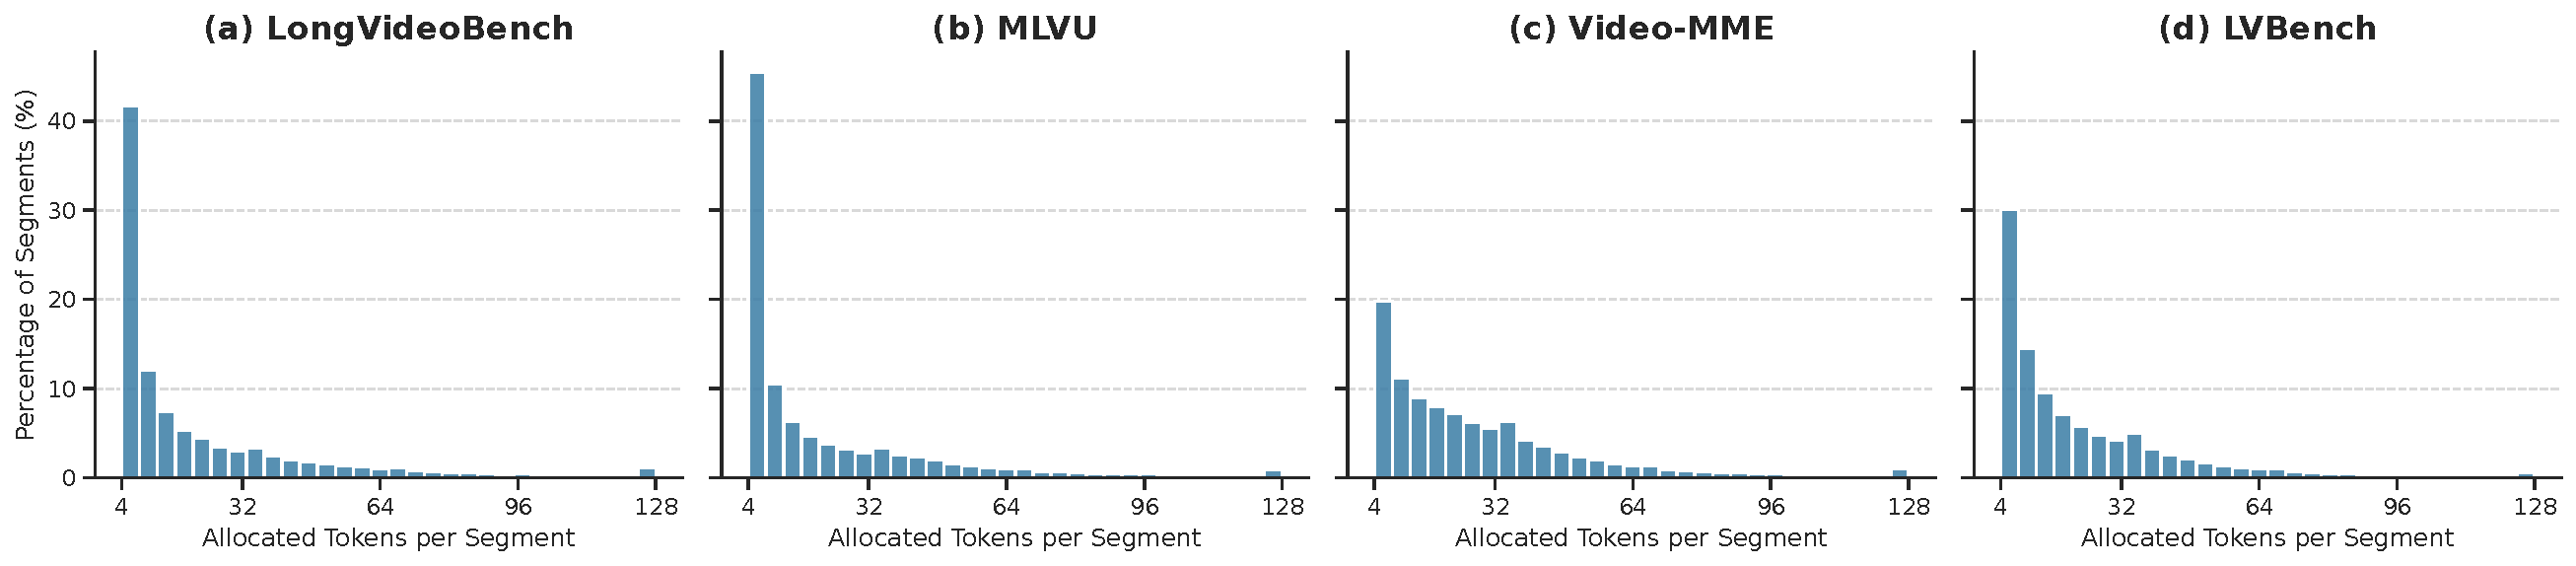
\includegraphics[width=0.95\linewidth]{supp/fig/token_overall_allocation_4k.pdf}
        \vspace{-0.5em}
    \end{subfigure}
    \\ \vspace{1em}
    % 8K
    \begin{subfigure}{\textwidth}
        \centering
        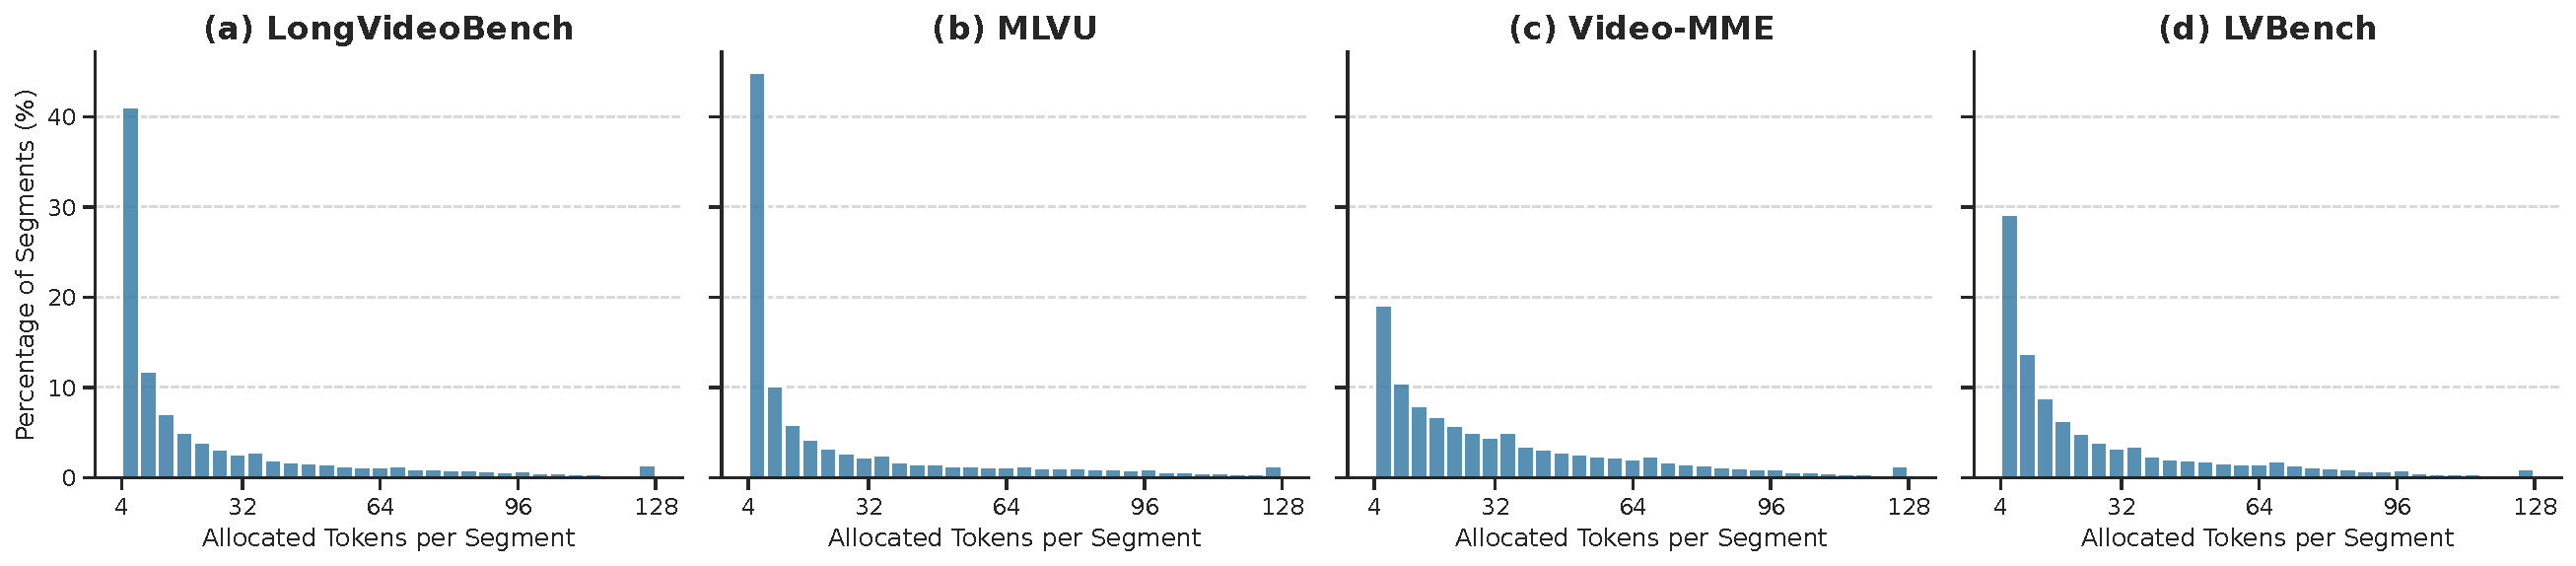
\includegraphics[width=0.95\linewidth]{supp/fig/token_overall_allocation_8k.pdf}
        \vspace{-0.5em}
    \end{subfigure}
    \caption{
        \textbf{Distribution of allocated tokens per segment.}
        \textbf{(Top)} 4K budget ($B=4096$); \textbf{(Bottom)} 8K budget ($B=8192$).
        Across four benchmarks, ATA consistently exhibits a strongly right-skewed, long-tailed allocation pattern. The majority of segments are compressed into very low-token representations, while a small fraction receives substantially higher allocations for query-aligned segments. Notably, this distribution pattern remains stable under different global budgets.
    }
    \label{fig:micro_dist}
\end{figure}
\begin{figure}[t]
    \centering
    % 4K
    \begin{subfigure}{\textwidth}
        \centering
        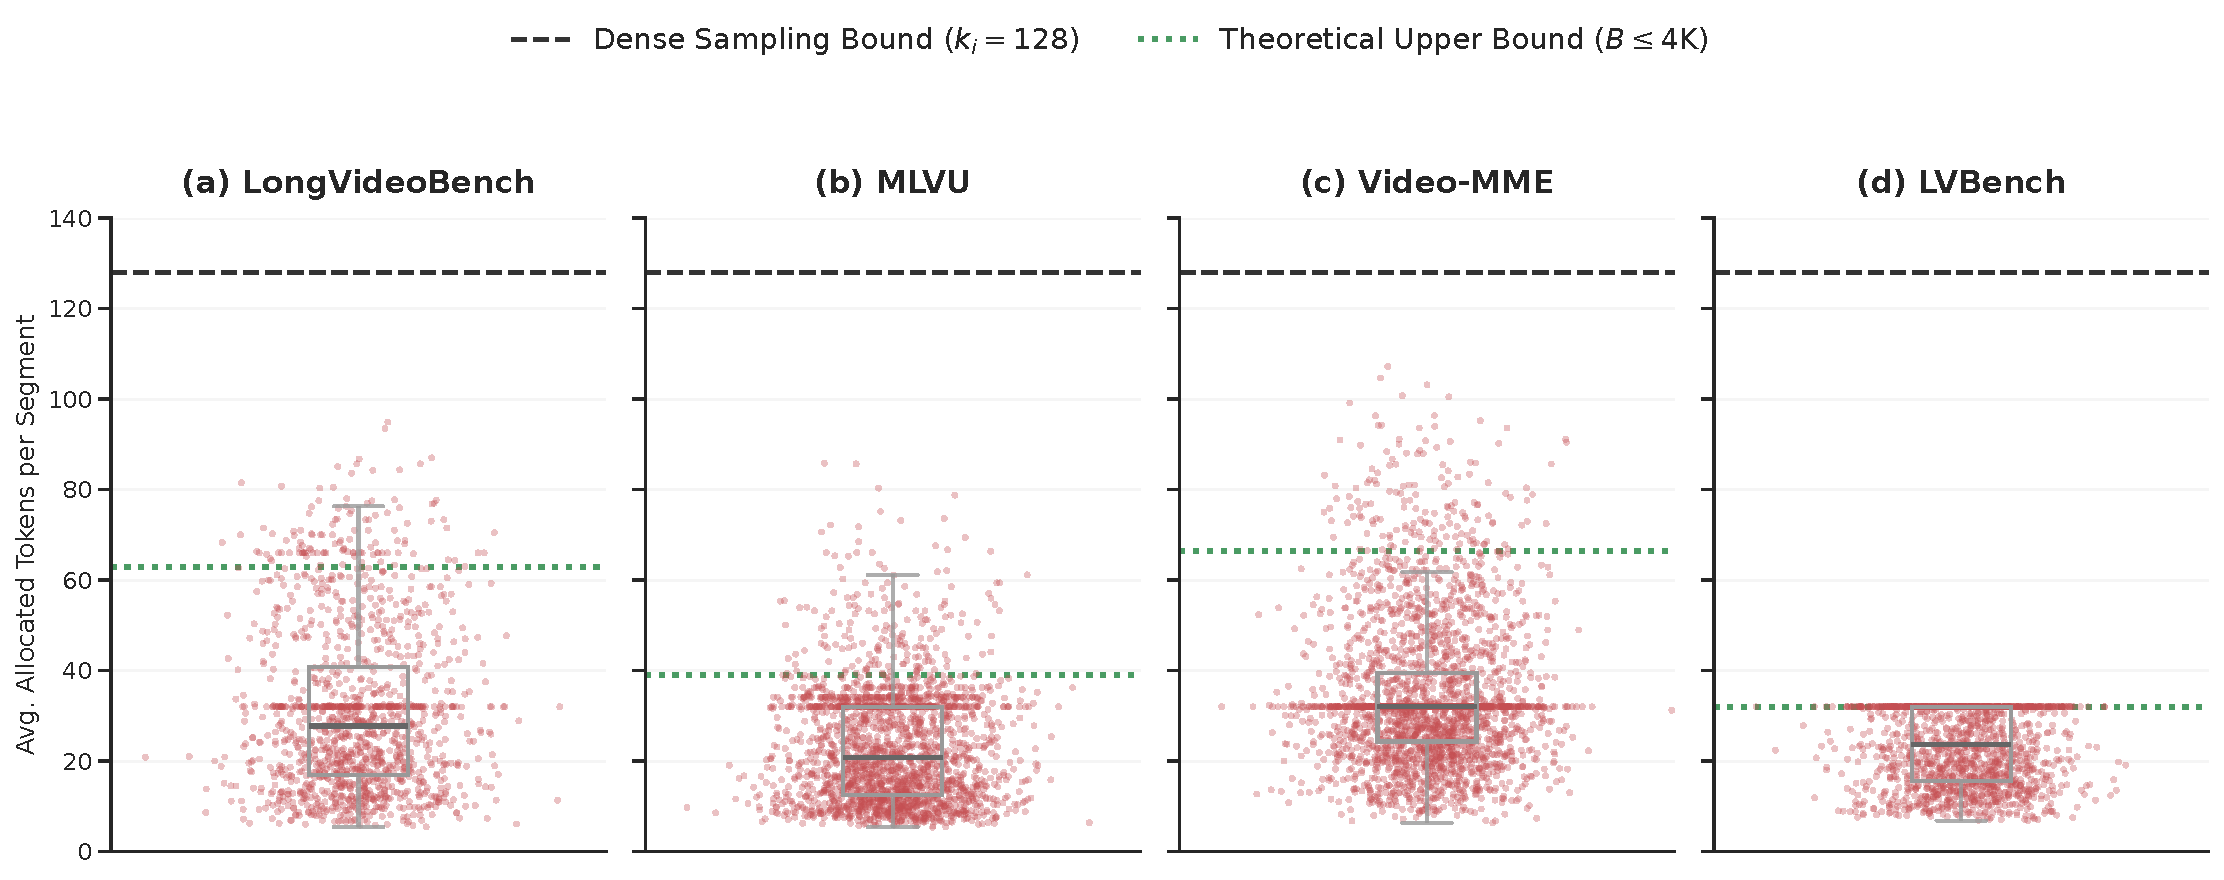
\includegraphics[width=0.95\linewidth]{supp/fig/token_consumption_rigorous_4k.pdf}
        \vspace{-0.5em}
    \end{subfigure}
    \\ \vspace{1em}
    % 8K
    \begin{subfigure}{\textwidth}
        \centering
        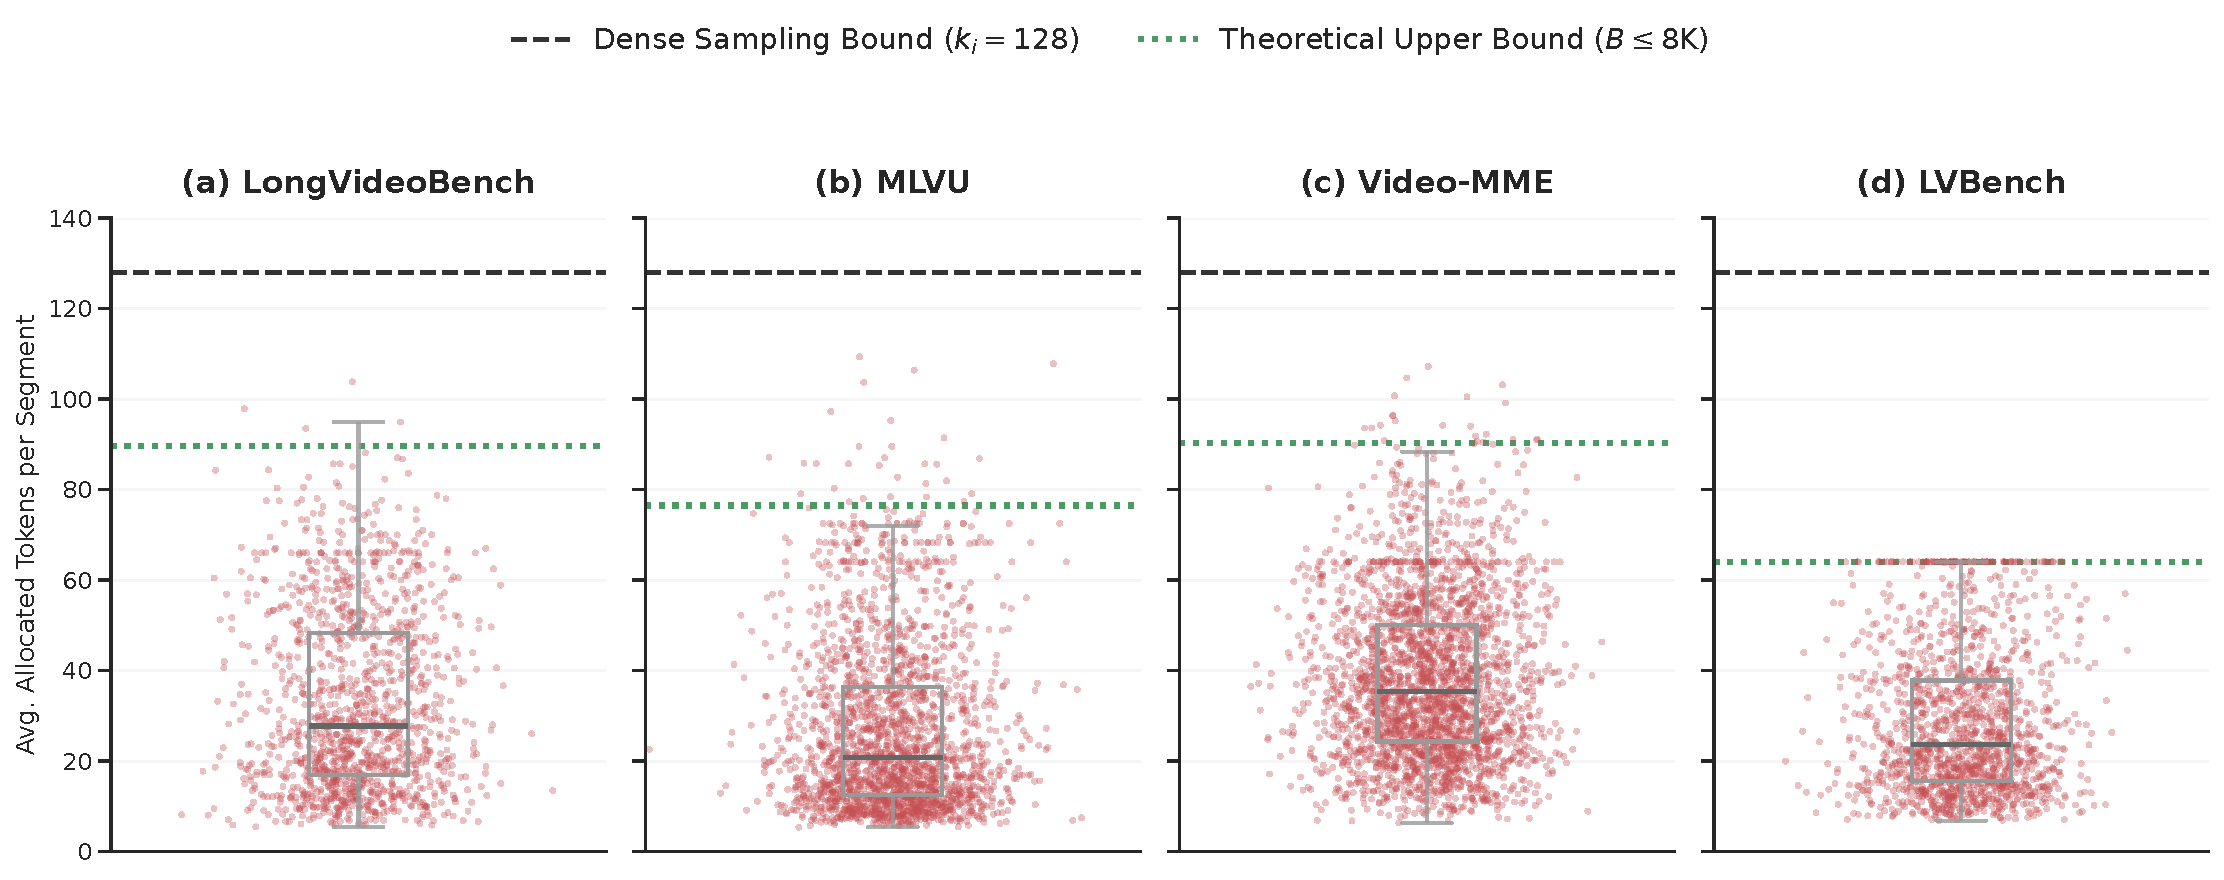
\includegraphics[width=0.95\linewidth]{supp/fig/token_consumption_rigorous_8k.pdf}
        \vspace{-0.5em}
    \end{subfigure}
    \caption{
        \textbf{Macro-level budget utilization and adaptation efficiency.}
        \textbf{(Top)} 4K budget; \textbf{(Bottom)} 8K budget.
        Each red dot denotes the \emph{average token consumption per segment} for a video sample. The dashed green line indicates the \emph{dataset-level average theoretical capacity}. Points above the line correspond to shorter videos whose per-segment capacity is higher than the dataset-wide average.
        \textbf{Adaptability:} On datasets with diverse video lengths (\eg, LongVideoBench, Video-MME), the consumption distribution remains well below the theoretical capacity, indicating query-driven compression.
        \textbf{Reliability:} On extremely long videos (LVBench), the token consumption forms a clear ceiling at the theoretical limit, demonstrating strict adherence to the global budget constraint.
    }
    \label{fig:macro_efficiency}
\end{figure}